\documentclass[a4paper,10pt]{article}
\usepackage[utf8]{inputenc}
\usepackage{graphicx}\usepackage{listings}

\usepackage{graphics}


\begin{document}
\thispagestyle{empty}
Potential field solution when the potential at the surface of the cylinder is $V_0$, the radius is $a$, and the field strength is $E_0$:
\[ \Phi(r, \theta) = V_0 + E_0 cos\theta \left( \frac{a^2}{r} - r\right) \]
\begin{figure}[h!]
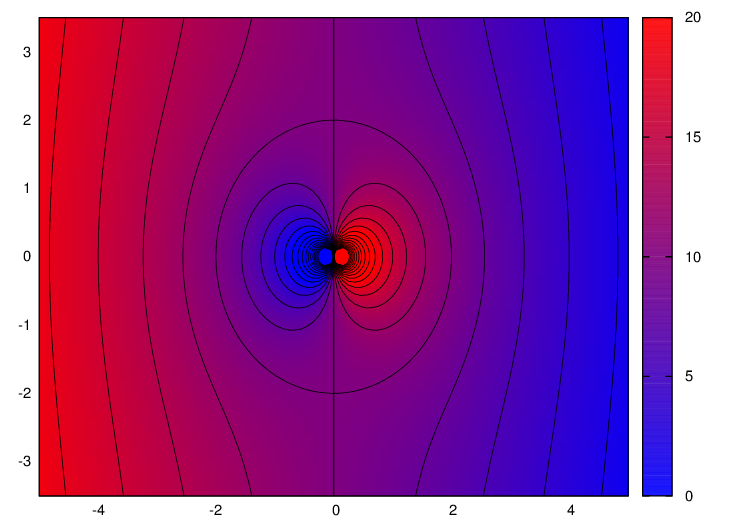
\includegraphics[width=\textwidth]{potential.png}
\caption{Shape of potential (scalar) field when $a = 2$, $E_0 = 2$, and $V_0 = 10$. Electric field lines are perpendicular to the drawn
contour lines.}
\end{figure}


Electric field (set $E_0 = a = 1$):
\[ E(x,y) = - \nabla\Phi(x,y) = \left(\frac{2 x^2}{(x^2+y^2)^2}-\frac{1}{x^2+y^2}+1\right)\underline{i} + \frac{2 x y}{(x^2+y^2)^2}\underline{j} \]

\vspace{1cm}

Problem: take care of singularity inside conductor (potential field should be constant inside conductor). Define it piecewise?

\vspace{1cm}

Question: is $V_0$ a function of $E_0$ since we know the cylinder is a perfect conductor?
\end{document}